\section{Introduction}
\label{sec:introduction}

Vision-Language-Action (VLA) models~\cite{Kim2024OpenVLA, OctoModelTeam2024} degrade under deployment-time distribution shifts in environment appearance, object geometry, or instruction phrasing, and recovering reliable behavior requires adaptation~\cite{Ferchau2026VLALoRA}.
Every deployment site presents its own shift, so adaptation repeats across sites, and each instance operates in a low-data regime, typically tens of demonstrations collected on the robot.
Full fine-tuning is ill-suited to this regime, as it optimizes billions of parameters against a demonstration set more than eight orders of magnitude smaller, and in our experiments it overfits even at its best validation checkpoint and degrades the held-out-scene generalization of the pretrained policy.
The dominant strategy applies parameter-efficient fine-tuning (PEFT) methods such as Low-Rank Adaptation (LoRA)~\cite{Hu2022LoRA} uniformly across all layers at a fixed global rank, which implicitly assumes that every network region requires equal adjustment.
A VLA, however, comprises functionally distinct regions, namely a vision encoder, a language backbone, cross-modal projectors, and an action head, and a perturbation confined to one input modality need not implicate every region.
Biological sensorimotor control exhibits the same structure, as the nervous system is thought to maintain separable internal models and to update only those whose predictions fail~\cite{Wolpert1998MOSAIC}.
When a shift implicates only a subset of regions, uniform allocation overprovisions the unimplicated regions and underprovisions the implicated ones.

\begin{figure}[!tp]
    \centering
    \setlength{\abovecaptionskip}{4pt}
    \setlength{\belowcaptionskip}{-10pt}
    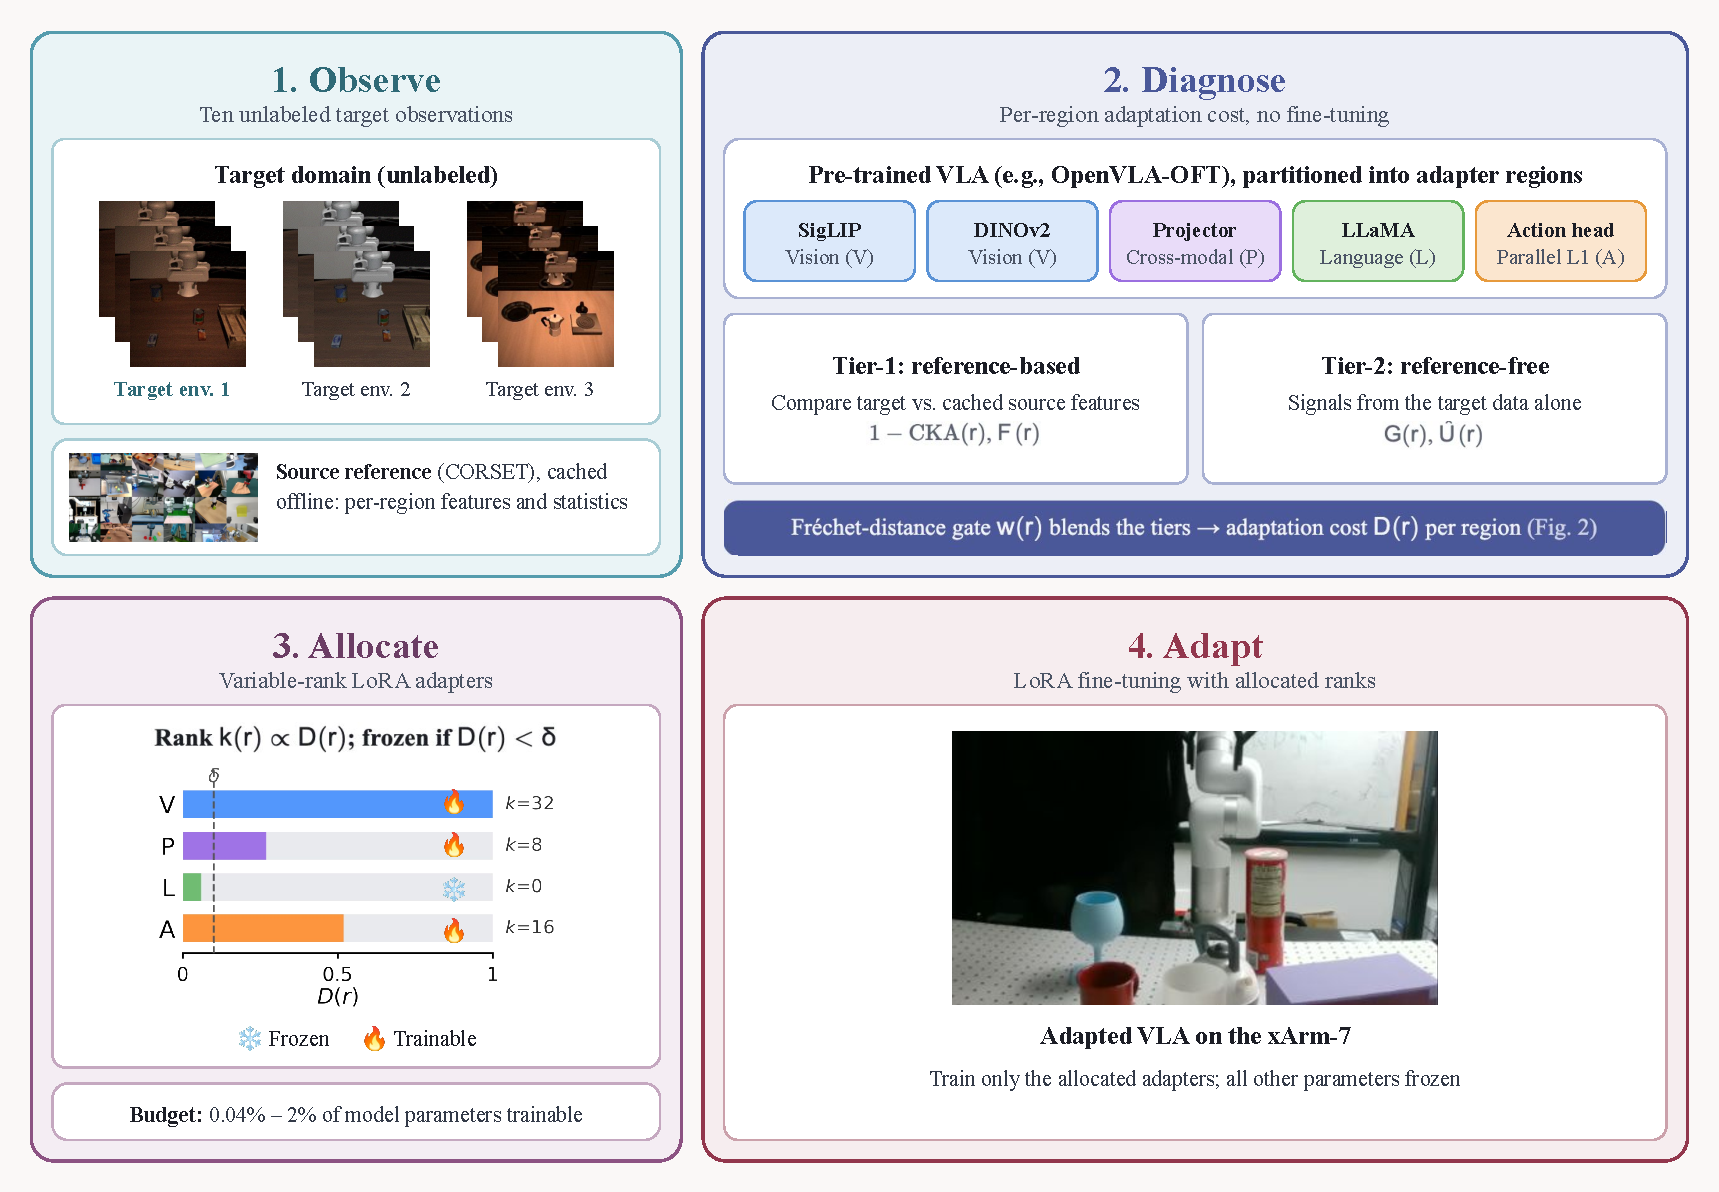
\includegraphics[width=\columnwidth]{images/interpretability_figure1.pdf}
    \caption{\textbf{Observe, diagnose, allocate, adapt.} From a few unlabeled target observations, the pipeline estimates per-region adaptation cost using Tier-1 reference-based signals, Tier-2 reference-free signals, and a Fr\'echet-distance gate to blend them. A budget-aware allocator assigns variable-rank LoRA adapters and freezes well-calibrated regions, and the adapted policy matches full fine-tuning on the xArm-7 at a fraction of the trainable parameters.}
    \label{fig:system-overview}
\end{figure}

Selective adaptation has precedent in vision models~\cite{Lee2023Surgical, He2023SPT, Zhang2023AdaLoRA}, and concurrent work allocates non-uniform LoRA capacity during VLA fine-tuning~\cite{Kim2026LoRASP} or traces VLA representations after fine-tuning~\cite{Shi2026VLATrace}.
To the best of our knowledge, this is the first work to measure, before fine-tuning and from a small set of unlabeled target observations, how adaptation demand distributes across the functional regions of a VLA, and to convert that measurement into a capacity allocation.

This paper first characterizes that distribution empirically across five architecturally distinct VLAs under five controlled deployment shifts.
The resulting \emph{adaptation spectrum} concentrates adaptation cost in a shift-specific region, with the dominant region consistent across all five architectures in our experiments.
We then introduce a pipeline with four stages, which \emph{observes}, \emph{diagnoses}, \emph{allocates}, and \emph{adapts} (Fig.~\ref{fig:system-overview}, \S\ref{sec:method}).
We evaluate the pipeline on the LIBERO~\cite{Liu2023LIBERO} and CALVIN~\cite{Mees2022CALVIN} benchmarks and on a physical UFactory xArm-7 manipulator.
The diagnostic ranks regions within each deployment at a median Spearman correlation of $0.91$, and the allocation matches or exceeds uniform LoRA at every parameter budget we tested on all five architectures.
On the xArm-7, the pipeline matches full fine-tuning under an instruction-wording shift with 0.04\,\% of its trainable parameters, and on five held-out scenes evaluated without retraining it leads every baseline, with 11--23 successes of 30 against 8--18 for the strongest PEFT baseline at equal or larger budgets and 2--11 for full fine-tuning.
This paper makes three contributions.
\begin{enumerate}[itemsep=2pt, topsep=3pt, partopsep=0pt]
    \item An empirical characterization of how adaptation cost distributes across functional regions under five deployment shifts, with the dominant region per shift type consistent across five VLA architectures (93M--7B parameters) and three action-decoding paradigms.

    \item An algorithm that estimates per-region adaptation cost from ten unlabeled target observations without fine-tuning and converts the estimates into variable-rank LoRA adapters matching uniform rank-32 success rates at a reduced parameter count in our experiments.

    \item Experiments across five architectures, five seeds, and six physical deployment shifts that characterize where the allocation helps and include one negative result in which it does not.
\end{enumerate}